\section{Artificial Neural Network}\label{artificial-neural-network}

Le reti neurali sono una sottobranca dell'intelligenza artificiale, il
termine IA è stato coniato negli anni `50 ma ci sono origini ancora più
indietro. Esistono due filoni, uno per l'ottimizzazione delle macchine
per processare dati (Von Neumann) e uno chiamato cibernetica cioè creare
macchine copiando i sistemi nervosi degli esseri viventi.

Dalla cibernetica è nato il machine learning cioè sistemi che hanno
un'efficacia che migliora nel tempo, in soldoni ``imparano''.

\subsection{Neuroni}\label{neuroni}

Le reti neurali sono basate dai collegamenti dei neuroni nel nostro
cervello, un sistema nervoso è più veloce in operazioni input e output
(grazie ai collegamenti) invece il computer nel tempo di processamento.

I neuroni fisici cono cellule, ma con una struttura differente rispetto
ad altre, con una parte allungata (assone) che rappresenta l'output.

Per scambiare dati usano l'elettricità tramite la differenza tra ioni
esterni e interni. Infatti il voltaggio rapido colpendo la parete
cellulare la fa lavorare al contrario e ogni parte della membrana eccita
quella di fianco e permette di trasportare il segnale; arrivato alla
fine del neurone il segnale si propaga al più vicino tramite i
neurotrasmettitori.

C'è la possibilità di sommare diversi segnali deboli in uno più forte,
la somma può essere temporale o spaziale.

\subsection{Modelli}\label{modelli}

Nei modelli neurali abbiamo i seguenti elementi:

\begin{itemize}
\item
  Neuroni con canali di input finiti;
\item
  Ogni canale ha un peso, un valore numerico (identifica l'efficacia
  della comunicazione);
\item
  Una soglia per ogni neurone;
\item
  Diversi stati per ogni neurone (mapping fra ingressi e uscite) con un
  modello matematico.
\end{itemize}

\subsubsection{Binary threshold neuron}\label{binary-threshold-neuron}

Il primo modello creato da McCulloch e Pitts nel `43.

I loro neuroni, con la loro soglia, usano segnali binari e hanno tante
entrate e una sola uscita. In ogni istante ogni neurone fa la somma
pesata degli ingressi e la controlla con la soglia, se \textgreater= 1
esce un segnale 1 altrimenti 0.

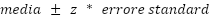
\includegraphics[width=3.09375in,height=1.21875in]{media/image1.png}

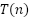
\includegraphics[width=6.26772in,height=1.33333in]{media/image5.png}

Se per esempio abbiamo una soglia di 5 e abbiamo due ingressi entrambi
di valore 3 ma pesati 1 e 0 il valore di uscita sarebbe 0 perchè 3*1 +
3*0 \textless{} 5.

Questo modo di rappresentare i neuroni è computalmente universale, cioè
puoi fare tutto, questo perchè è possibile rappresentare AND OR NOT:

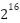
\includegraphics[width=6.26772in,height=3.34722in]{media/image3.png}

\subsubsection{Problema dello XOR}\label{problema-dello-xor}

I neuroni appena visti non riescono a rappresentare lo XOR, questo
perché un singolo neurone non riesce a far altro che dividere gli input
tramite una linea, chi sta sopra e chi sotto.

\subsubsection{Percettroni}\label{percettroni}

L'idea era creare una retina artificiale per analizzare l'immagine, dove
ogni pixel veniva associato ad un input della rete neurale (demone) che
lo passa ad un livello inferiore che fa il calcolo come i neuroni
precedenti e \emph{identifica una feature}. \textbf{Ed è una rete a
livelli}.

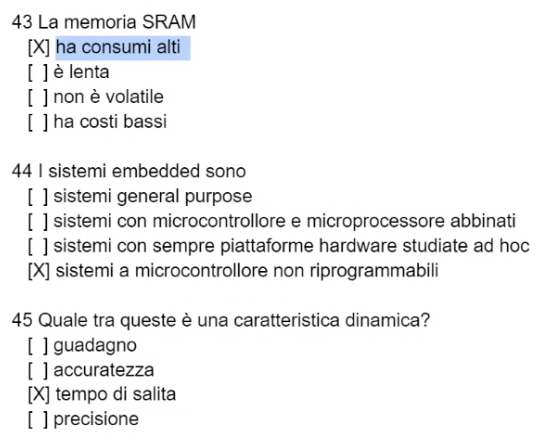
\includegraphics[width=5.17708in,height=3.22917in]{media/image8.png}

Più aggiungiamo livelli più l'analisi è precisa:

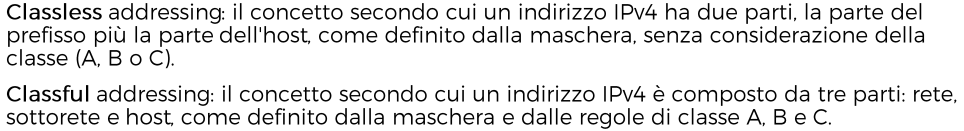
\includegraphics[width=6.26772in,height=3.88889in]{media/image6.png}

Con la rete a tre livelli posso fare tutto teoricamente.

Se suddivido troppo le regioni di classificazione (come nel terzo
livello) posso andare in \textbf{overfitting} e il modello al lungo
andare non riesce ad identificare i nuovi esempi perché le regioni sono
troppo precise.

Visto che ogni nodo aggiunto ad una rete deve essere settato e andando
avanti i nodi crescono tantissimi sono nati modelli che imparano da soli
a settare i nodi grazie ai training set.

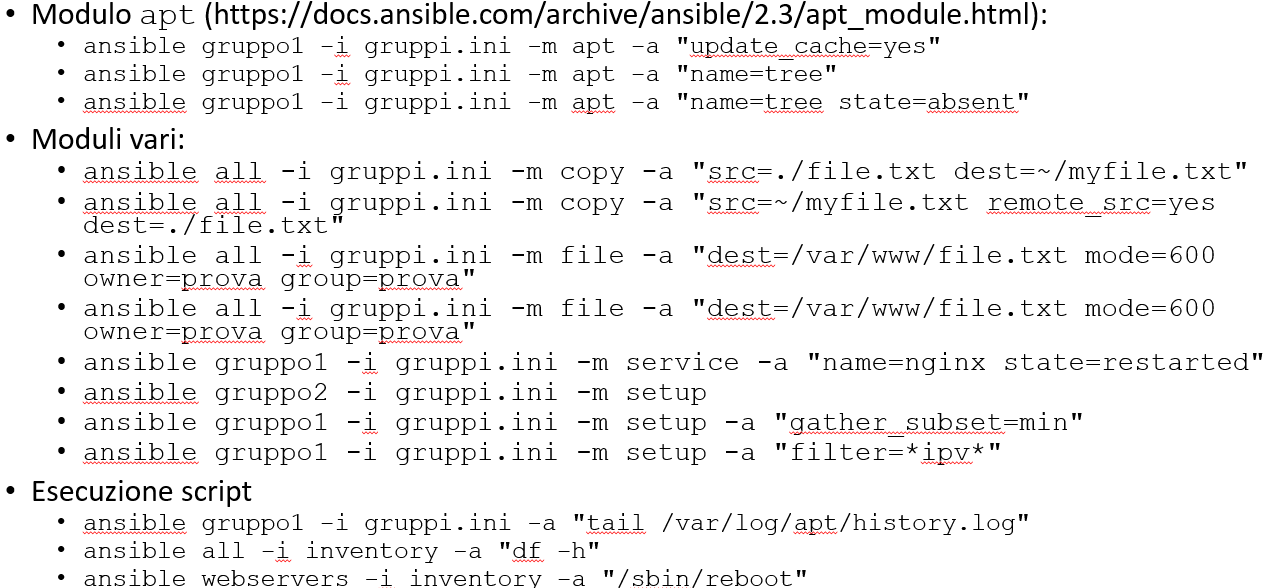
\includegraphics[width=6.26772in,height=2.5in]{media/image2.png}

Il primo modello di allenamento supervised è stato \textbf{Hebb's law},
che dice:

\emph{``If two units are active at the same time, the weight of their
connection must be increased''}

Ma non si riesce ad identificare il peso giusto per livelli separati.

Successivamente è nato il \textbf{Gradient descent} dove ad ogni input
associo un errore nell'output che viene rappresentato graficamente, più
è alto il punto nel grafico più l'errore è massiccio, successivamente
cerco la funzione che ha l'errore più piccolo.

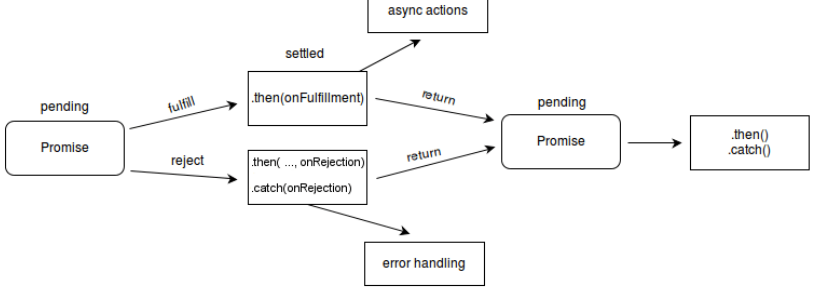
\includegraphics[width=6.26772in,height=3.66667in]{media/image7.png}

Nel grafico le ``vallate'' sono i risultati dove si sono ottenuti
risultati migliori e il nostro scopo è trovare la ``strada'' che dalla
cima porta alla valle in maniera più veloce.

Il \textbf{Back propagation} è un altro algoritmo che calcola il
gradiente dell'algoritmo precedente propagando il segnale
dall\textquotesingle output all'input.

Per farlo usa una funzione matematica che è facilmente implementabile
con uno script.

La funzione di \textbf{attivazione} definisce l'output che i nodi danno
ad un certo input, permette di usare più numeri dei soli 0/1, ne
esistono tre principali:

\begin{itemize}
\item
  \textbf{Sigmoid}: passando un valore reale otteniamo un output che
  varia tra 0 e 1;
\item
  \textbf{Tanh}: come prima ma l'output varia tra -1 e 1;
\item
  \textbf{reLU}: l'output è una funzione non lineare degli input totali.
  Se il valore passato è sotto o uguale a 0 non viene calcolato
  altrimenti passa la parte positiva.
\end{itemize}

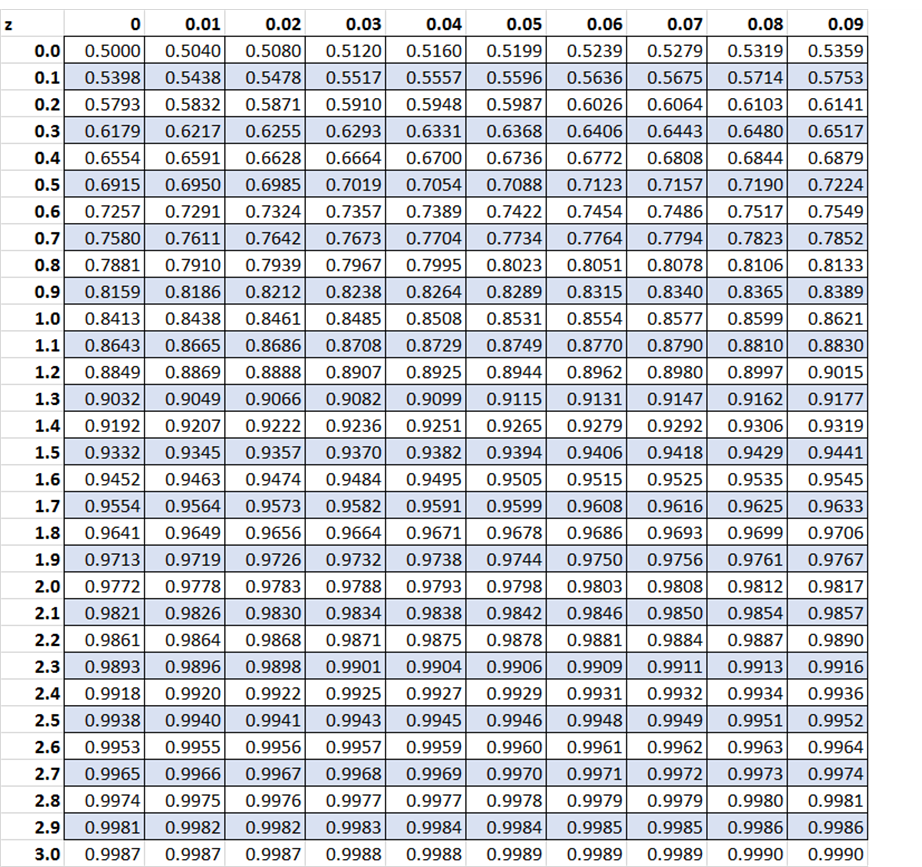
\includegraphics[width=6.26772in,height=3.375in]{media/image9.png}

Il \textbf{Deep learning} o \emph{hierarchical learning} usa una rete a
più livelli per estrarre caratteristiche complesse dai dati, lo scopo
principale è evitare l'identificazione manuale di caratteristiche
astratte grazie ad algoritmi di allenamento non supervisionati o semi
supervisionati.

Le caratteristiche principali sono:

\begin{itemize}
\item
  sequenza di livelli di processione non lineare per estrarre le
  caratteristiche;
\item
  ogni livello rappresenta un diverso livello di astrazione.
\end{itemize}

Una \textbf{deep neural network}, è una rete neurale con tanti livelli
nascosti, possono modellare relazioni complesse e non lineari.

La successione di livelli permette la composizione delle caratteristiche
identificate dai livelli inferiori.

Nel 2006 è stato finalmente stato trovato un algoritmo di addestramento
efficace per queste reti, il \textbf{Greedy Layer Wise Training}, cioè
l\textquotesingle addestramento della rete strato per strato in modo
sequenziale, utilizzando l\textquotesingle output di ogni strato
allenato come input per lo strato successivo.

Ecco gli step:

\begin{enumerate}
\def\labelenumi{\arabic{enumi}.}
\item
  Addestramento del primo livello nascosto (``Features'') e
  ricostruzione dell'input basandosi sull\textquotesingle output del
  livello nascosto; con calibrazione del peso al contrario fino al
  livello input.
\item
  Addestriamo il livello successivo (``Additional Features'') con
  l'output del livello ``Features''; con calibrazione del peso al
  contrario fino al livello Features.
\item
  Continuiamo con questo metodo fino al livello output e calibriamo i
  pesi fino all'input level.
\end{enumerate}

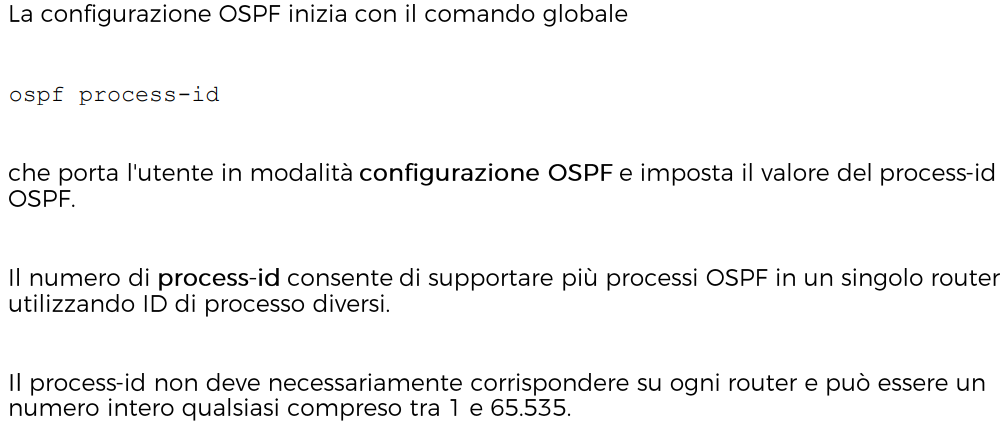
\includegraphics[width=5.16146in,height=1.84338in]{media/image4.png}

L'avvento delle GPU sul mercato e il loro successivo miglioramento ha
portato a diminuire i tempi di calcolo degli algoritmi di allenamento,
questo perché le GPU sono perfette per il calcolo vettoriale.
